\appendix
\chapter{Implementation}
\section{Logo Activity}
\begin{figure}[h!]
	\centering
	
\includegraphics[scale=0.3]{gfx/logo-activity_1.jpg}
	\caption{Portrait Logo Activity only shown when user do not have a valid session.}
	\label{fig:logo-activity_1}
\end{figure}
\begin{figure}[h!]
	\centering
	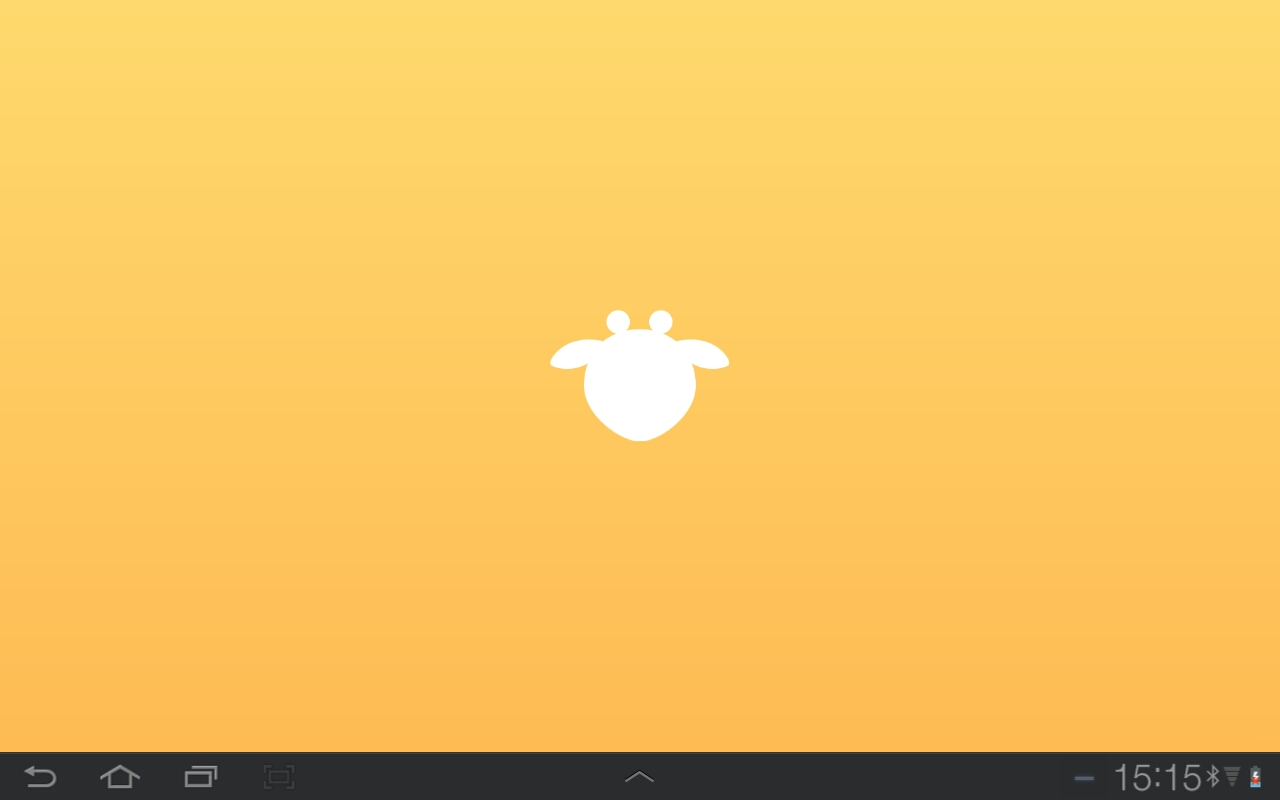
\includegraphics[scale=0.3]{gfx/logo-activity_2.jpg}
	\caption{Landscape Logo Activity only shown when user has an valid session in and start the application again.}
	\label{fig:logo-activity_2}
\end{figure}
\section{Profile select activity}
\begin{figure}[h!]
	\centering
	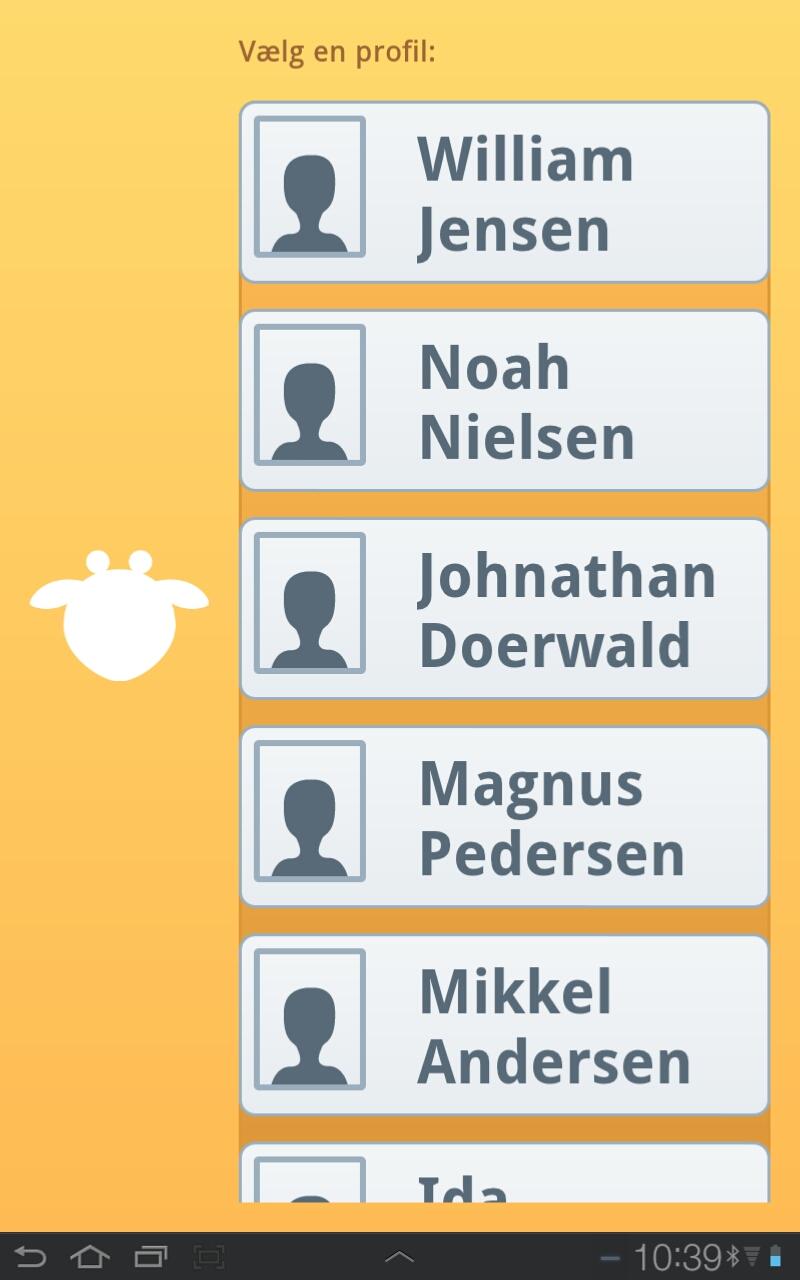
\includegraphics[scale=0.3]{gfx/profile-select-activity_1.jpg}
	\caption{Portrait profile select activity screenshot}
	\label{fig:profile-select-activity_1}
\end{figure}

\chapter{Usability - Use Cases}
\label{appendix_use_cases}

\section{New Guardian Log in}
Karen is new at her workplace where she has had her GIRAF profile created already and is now trying to use a GIRAF tablet for the first time. 
She has recieved her authentication QR code, and after she has booted the tablet up, it prompts her to scan her QR code. 
She presses accept and is sent to the QR code app, where she scans her code and is sent back to the GIRAF system after it has scanned her code. 
She is now in guardian mode and can access the children she has been authorized for.

\section{Configuring an app for a child}
The GIRAF systems where Karen works have recently received a new app that she wants to use with one of the kids. 
To prepare, she has the tablet she is logged in on and wants to open the settings app to personalize the app ahead. 
When she opens the app, she is given a list of profiles where she chooses the profile for the child.
The settings app then becomes active, and displays a list of all apps that are available to the child, and the bottom the app has a button for adding more apps to the list. 
She presses that button and receives a list of all available apps on the system. 
She then finds the new app, selects it and confirms that she wishes to make this app available to this child.
She is then sent back into the settings app with the list of apps where she can now choose the new app. 
She does so, and the settings app opens a page next to the list where she is asked to change settings in "`text"' mode or in snapshot mode.
She first chooses "`text"' mode, and receives a list of the settings she can change in the app. 
She wants to change the background color of the app, so she finds the setting labelled "`Baggrund"', presses it and is given the option of choosing a picture or a color as background. 
She selects color and is given the option of choosing the color from a color wheel. 
She marks the desired color and presses "`OK"' (which means her new settings have been saved).
She wants to change other aspects of the app as well, but prefers doing so in snapshot mode, so in the list of apps available to the child, she presses the app again, and now selects snapshot mode when prompted.
An interactive snapshot of the given app is now opened next to the list of apps, and pressing elements of the app allows her to configure them. 
She presses an element she would like to resize and does a pinching motion to make the element smaller. 
She then presses the "`OK"' button (which means her settings have been saved) at the bottom of the screen and is returned to the interactive snapshot's starting state.
She is finished editting the settings of the app and so she presses the Home button and is returned to her launcher.

\section{Launching an app for a child in Guardian mode}
Karen is trying to work with a child and wants to open an app with that child's profile. 
In guardian mode, she presses the icon for the given app and receives a list of profiles to launch the app with. 
The child's profile is not directly visible, so she scrolls down the list until she finds the correct profile. 
She selects the profile and the app then launches with the settings specified for that profile.

\section{Letting a child use an app for a limited time}
Karen wants to let a child use an app in the child's break. 
With the system in guardian mode, she presses the icon for the app. 
A list of profiles then pops up, and by swyping in from the left, a list of apps that can interact with the app becomes visible. 
With a time app installed, it is visible on the list and allows Karen to choose a period of time where the app it is used with will become unavailable after this time runs out.

\chapter{QR codes}
\section{QR code test}
\begin{figure}[h!]
	\centering
	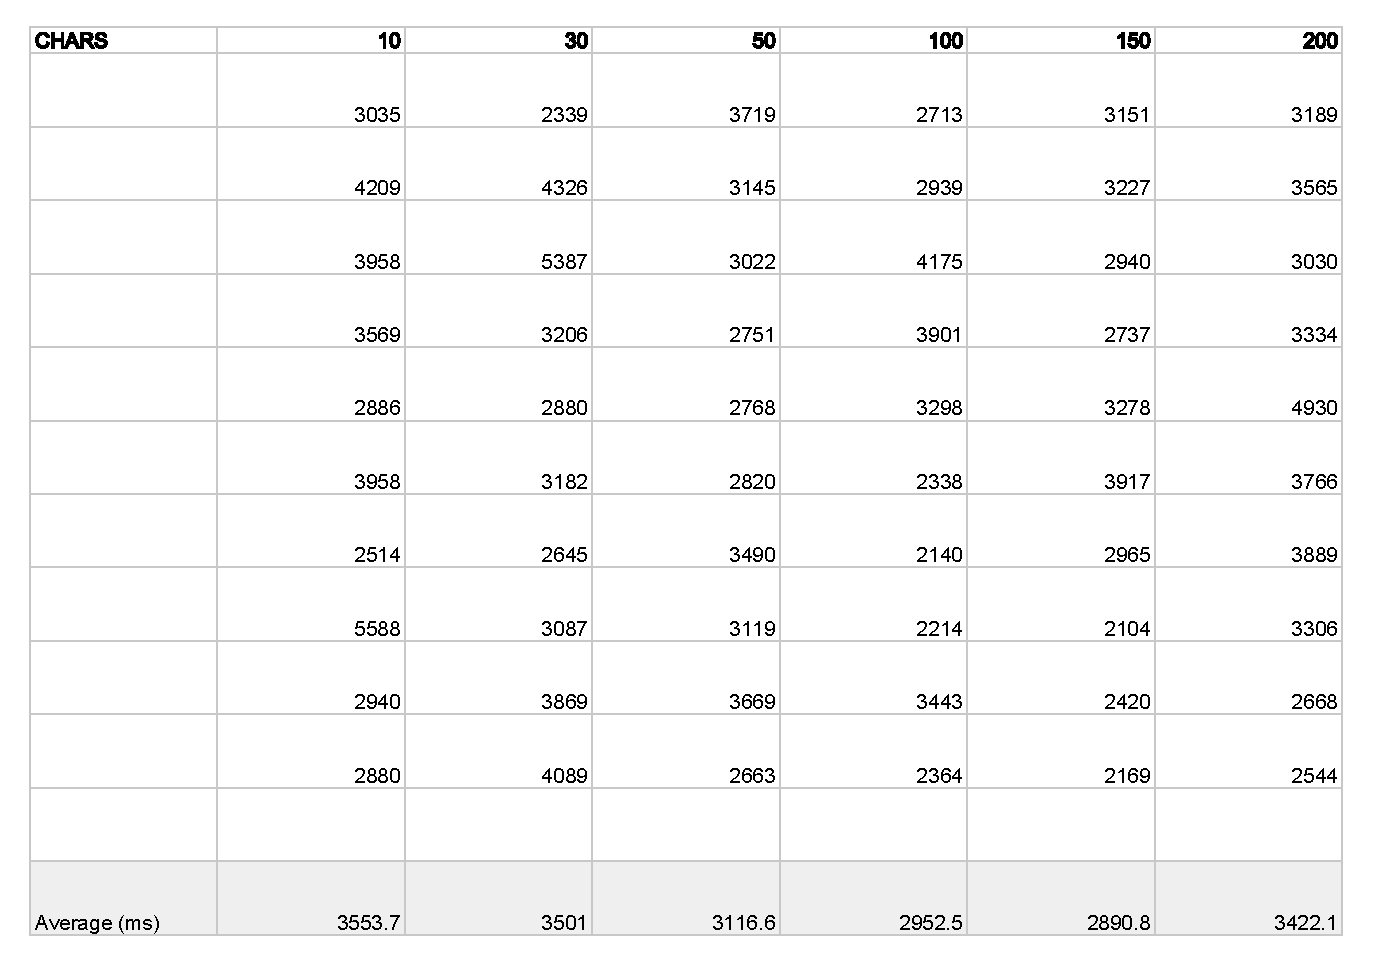
\includegraphics[scale=0.3]{gfx/QR-test.pdf}
	\caption{The results from the QR code test, all times are in ms}
	\label{fig:QR-code-test}
\end{figure}
